
\section{Dynarobin leg model}

This paper goal is to improove locomotion stability on quadrupedal robot Dynarobin, depicted in Fig. \ref{fig:Dynarobin}. Dynarobin has four identical legs, each combning three rotational joints: shoulder, elbow, and wrist, respectively. Additionally each leg containts mehanical spring which defines stiffnes to the contact surface. In order to obtain spring-mass compliante leg behavior, impedance or simillar torque based control can be used. The aproximative Dynarobin leg model is shown in \ref{fig:DynarobinLEG}. It consists of three masses connected by one virtual active and one passive spring. 
\begin{figure}
	\centering
	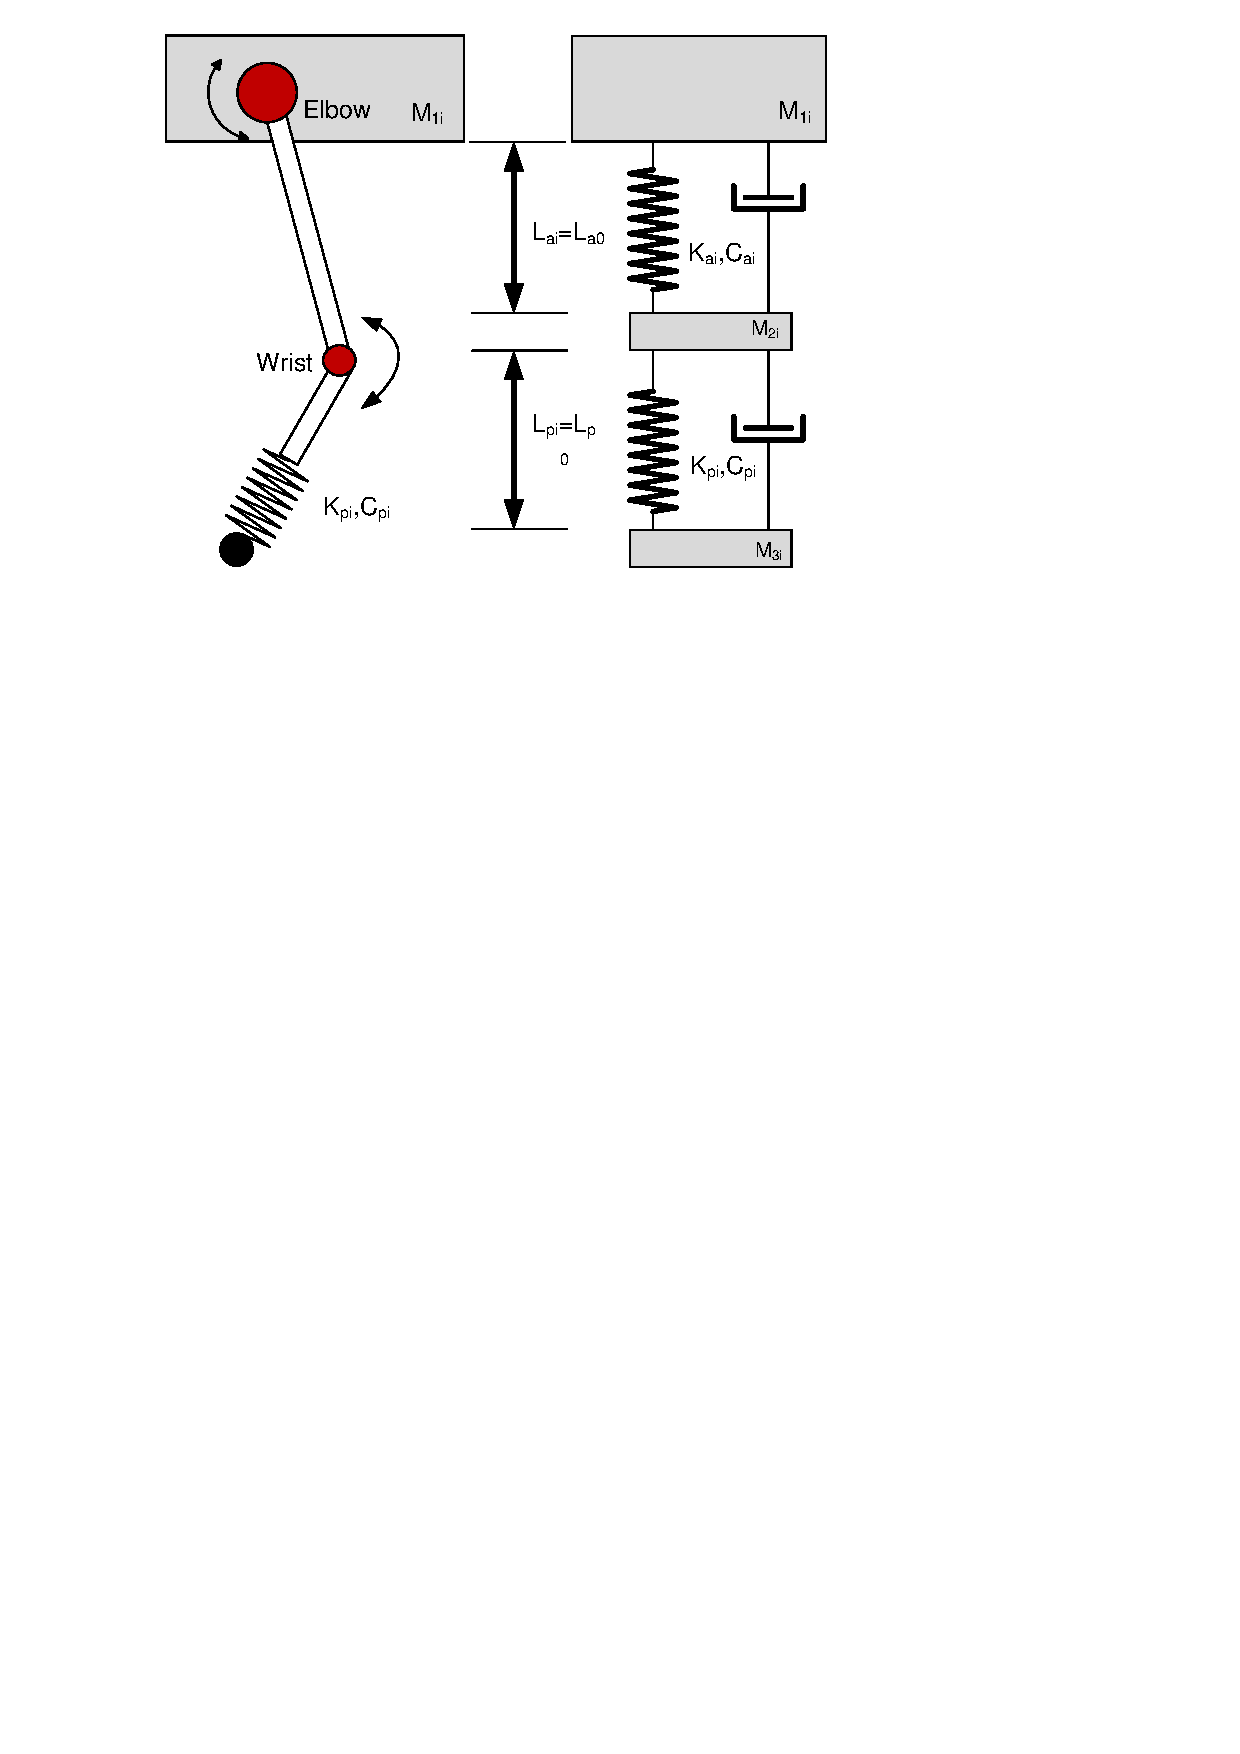
\includegraphics[width=75mm]{./pictures/Dynarobin_leg.pdf}
	\caption{Dynarobin leg model}
	\label{fig:DynarobinLEG}
\end{figure}
